\documentclass[12pt]{article}
\usepackage{amsmath, amssymb}  % Add useful math symbols and environments
\usepackage{amsfonts}          % Add fonts for sets like \mathbb{Z}
\usepackage{enumitem}          % Better control of list formatting
\usepackage[amsthm,thmmarks]{ntheorem} %Proof formatting
\newcommand{\Z}{\mathbb{Z}}    % Custom command for integers
\newcommand{\sset}{\subseteq}  % Custom command for subset notation
\newcommand{\Id}{\mathrm{Id}} % Custom command for identity
\usepackage{graphicx}
\usepackage{tikz}
\newcommand{\drawsquare}[2]{\filldraw[black!40!white] ({#1},{#2}) -- ({#1+1},{#2}) -- ({#1+1},{#2+1}) -- ({#1},{#2+1}) -- ({#1},{#2});}
\newcommand{\drawL}[2]{\draw[cyan,line width=1.5mm] ({#1},{#2}) -- ({#1+3},{#2}) -- ({#1+3},{#2+1}) -- ({#1+1},{#2+1}) -- ({#1+1},{#2+3}) -- ({#1},{#2+3}) -- ({#1},{#2});}

\begin{document}

\begin{center}
	{\LARGE Discrete Math - Homework 8} \Large \newline
    Name:
    % Write your name here.
\end{center}

\emph{Instruction summary:} Your work must be uploaded to Gradescope as a single PDF file. It must be typed in LaTeX to avoid a 20\% penalty. The polished proof must start in a new page (\textbackslash{newpage}). It will be graded based on clarity (2 points), LaTeX prowess (2 points) and proof quality (6 points, including for example structure and variable definition).

%------------------------------
% EXERCISES
%------------------------------
\section*{Exercises:}

\begin{enumerate}

% QUESTION 1
\item \emph{(4 points)} For which of the following functions, say if it is 1-1 and/or onto? Prove or disprove each statement.

\begin{enumerate}
\item \( f : \mathbb{Z} \to \mathbb{Z} \) with \( f(n) = n^2 + 1 \) for \( n \in \mathbb{Z} \).\newline

% Write your answers to question 1a here.

\item \( f : \mathbb{Z} \to \mathbb{Z} \) with \( f(n) = n/2 \) if \( n \) is even, and \( f(n) = 0 \) if \( n \) is odd. \newline

% Write your answers to question 1b here.

\item \( f: \mathbb{N} \to \mathbb{N} \) with \( f(n) = 2^n \) if \( n \) is even and \( f(n) = n \) if \( n \) is odd. \newline

% Write your answers to question 1c here.

\item \( f : \mathcal{P}(\mathbb{Z}) \to \mathcal{P}(\mathbb{Z}) \) with \( f(A) = A \cup \{ 0 \} \) for \( A \in \mathcal{P}(\mathbb{Z}) \). \newline

% Write your answers to question 1d here.
\end{enumerate}


% QUESTION 2
\item \emph{(3 points)} Show that the following functions are bijections. For each of them, give its inverse.

\begin{enumerate}
\item \( f : \mathbb{Z} \to \mathbb{Z} \) with \( f(n) = n + 1 \) for \( n \in \mathbb{Z} \). \newline

% Write your answers to question 2a here.

\item \( f : \mathbb{Z} \to \mathbb{N} \) with \( f(n) = 2n \) if \( n \geq 0 \) and \( f(n) = - 2n - 1 \) if \( n < 0 \). \newline

% Write your answers to question 2b here.

\item \( f : \mathcal{P}(\mathbb{Z}) \to \mathcal{P}(\mathbb{Z}) \) where \( f(A) = A \cup \{ 0 \} \) if \( A \in \mathcal{P}(\mathbb{Z}) \) does not contain 0, and \( f(A) = A - \{ 0 \} \) otherwise. You do not need to prove ``obvious'' results about sets, but your proof that the function is a bijection should still be totally rigorous. \newline

% Write your answers to question 2c here.
\end{enumerate}


% QUESTION 3
\item \emph{(4 points)} Fix \( b \in \mathbb{N} \).

Consider sets \( A, B, C \), and functions \( f : A \to B \) and \( g : B \to C \).

\begin{enumerate}
\item Show that if \( g \circ f \) is 1-1, then \( f \) is 1-1. \newline

% Write your answers to question 3a here.

\item Show that if \( g \circ f \) is onto, then \( g \) is onto. \newline

% Write your answers to question 3b here.

\item Consider two functions \( u : A \to C \) and \( v : C \to A \). Assume that \( v \circ u = \Id_A \) and \( u \circ v = \Id_C \). Show that \( u \) is a bijection and that \( v = u^{-1} \). \newline

% Write your answers to question 3c here.

\item Assume that \( f \) and \( g \) are bijective. Show that \( g \circ f \) is bijective and that \( (g \circ f)^{-1} = f^{-1} \circ g^{-1} \). \newline

% Write your answers to question 3d here.
\end{enumerate}



% QUESTION 4
\item \emph{(4 points)} 

\begin{enumerate}
\item Consider an equilateral triangle of size length 1. Show that if there are 5 points inside the triangle, then at least two of them are at distance less than or equal to \( 1/2 \). \newline

% Write your answers to question 4a here.

\item Consider a \( 8 \times 8 \) chessboard, with each square colored either black or white. Show that there must be two L-regions that are colored identically. Here, a L-shaped region consists of 5 adjacent squares shaped like an L, as in the picture below. \newline
\begin{center} %% This is tikz. All of the code below is to draw the figure. Don't change any of it!
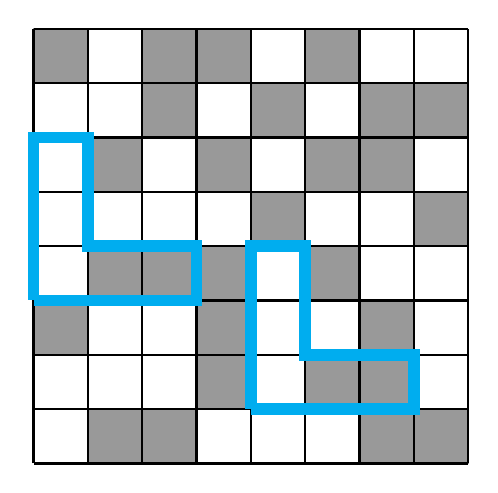
\begin{tikzpicture}[scale=0.69]
            \drawsquare{0}{7}\drawsquare{2}{7}\drawsquare{3}{7}\drawsquare{5}{7}\drawsquare{2}{6}\drawsquare{4}{6}\drawsquare{6}{6}\drawsquare{7}{6}
            \drawsquare{1}{5}\drawsquare{3}{5}\drawsquare{5}{5}\drawsquare{6}{5}\drawsquare{4}{4}\drawsquare{7}{4}\drawsquare{1}{3}\drawsquare{2}{3}
            \drawsquare{3}{3}\drawsquare{5}{3}\drawsquare{0}{2}\drawsquare{3}{2}\drawsquare{6}{2}\drawsquare{3}{1}\drawsquare{5}{1}\drawsquare{6}{1}
            \drawsquare{1}{0}\drawsquare{2}{0}\drawsquare{6}{0}\drawsquare{7}{0} \draw[thick] (0,0) grid (8,8); \drawL{0}{3} \drawL{4}{1}
        \end{tikzpicture}
\end{center}

% Write your answers to question 4b here.

\item Consider 51 points in a square of side length 1. Show that there are three points that can be covered by a disk of radius \( \frac{\sqrt{2}}{10} \). You will need the following easy extension of the pigeonhole principle: if we put \( > 2n \) pigeons in \( n \) pigeonholes, then one pigeonhole contains at least 3 pigeons. \newline

% Write your answers to question 4c here.

\item The integers \( 1, 2, \dots, 10 \) are written around a circle, in any order. Show that there are 3 adjacent numbers whose sum is 17 or more. Hint: the pigeonhole principle does not work here! Use contradiction instead. \newline

% Write your answers to question 4d here.
\end{enumerate}



\end{enumerate}
\newpage %Please do not erase this line.

%------------------------------
% POLISHED PROOF
%------------------------------
\section*{Polished proof:} 

\emph{(10 points)} Prove that \( f : \mathbb{R} \to \mathbb{R} \) with \( f(x) = \frac{1}{x} \) if \( x \neq 0 \), and \( f(0) = 0 \) is a bijection.

\noindent \emph{Claim.}
% Write here the statement you intent to prove. E.g: "Claim: There is only one even prime number."

\begin{proof}
%Write your proof here.
\end{proof}


\end{document}